With the PEGylation process fully optimized, we took the first step towards immunolabeling a full 3D artificial cornea, namely immunolabeling of a monolayer of cells on a microscope cover slip. The cells used were human dermal fibroblasts (HDFs) that express $\alpha5\beta1$-integrin, the same surface protein that we are targeting on the corneal cells. Performing immunolabeling on the monolayer allows assessment of the efficacy of the indirect immunolabeling process only, disregarding the collagen and removing the financial and temporal costs of building a complete corneal construct.

\section{Structure of the Immunolabeling Experiment}
\label{structureoftheimmunolabelingexperiment}

Several different preparations were used to determine the efficacy of the immunolabeling process. Each of them removes one or more key components of the process, which should yield to very little increase in the scattering contrast. The 6 preparations and their expected outcomes are described in the table below.

\rowcolors{1}{}{lightgray} 
\begin{table}[htbp]
\begin{minipage}{\linewidth}
\setlength{\tymax}{0.5\linewidth}
\centering
\small
\begin{tabular}{lcccc} \toprule
Preparation Name&1ary Ab?&2ary Labeler?&+Scattering Expected?&+Fluorescence Expected?\\
\midrule
Cells Only&No&No&No&No\\
2 only&No&Secondary Ab&No&No\\
1--2&Yes&Secondary Ab&No&Yes\\
2Au&No&OPAb-Au-PS&No&No\\
1--2Au&Yes&OPAb-Au-PS&Yes&Yes\\
Au&No&Naked Au&See Below&No\\

\bottomrule

\end{tabular}
\end{minipage}
\end{table}


Only those preparations with both primary and secondary antibodies should see an increase in the fluorescence signal, demonstrating the specificity of the secondary-to-primary binding. The 2 only and 1--2 samples were necessary to rule out any effects the Au nanospheres might have on the process. Scattering increase should only appear in the 1--2Au sample, because only the 1--2Au sample has both the gold to increase scattering and the secondary-primary binding to keep the gold bound to the cells. The one exception to this is the naked Au sample, where van der Waals forces and the presence of the salt solution may cause the spheres to agglomerate and stick to both the cells and the cover slip, causing a scattering increase.

The cells were prepared according to the procedure found in \autoref{The6MarchImmunolabelingProtocol}; in brief, the procedure is

\begin{enumerate}
\item Fix cells with paraformaldehyde

\item Permeabilize with Triton-X

\item Label the nuclei with Sytox Green and the actin filaments with phalloidin (fluorescent stains)

\item Add primary antibody if appropriate for a given preparation

\item Add appropriate secondary labeler

\end{enumerate}

Each preparation had three different samples (except for 2Au, which had two) to minimize intrinsic variation during inter-preparation comparison. After labeling, each sample was imaged in three different places with the confocal microscope, using both fluorescence and backscattering modes, and then each sample was imaged at five different $500\,\mu\mathrm{m}\,\times\,500\,\mu\mathrm{m}$ field of view locations with the OCM (except for 2Au, for which each sample was sampled at 10 different locations).

\section{Results of the Immunolabeling Experiment}
\label{resultsoftheimmunolabelingexperiment}

Representative confocal images for each labeled sample are shown in \autoref{confocalcollage}. Comparison between the 2 only and 1--2 confocal images reveals trails of green dots away from the nucleus only in the 1--2 sample; this is the expected pattern of labeled integrins. The appearance of stained integrins in only the 1--2 preparation indicates that both the primary and secondary antibodies bind only to the integrin and primary antibody, respectively. The samples with gold, however, are not as encouraging. Appearance of distinguishable cellular features in the back-reflectance channel indicates that the gold spheres bind to the cells--and to the cover slip--regardless of the presence of either the primary or secondary antibody. Nevertheless, cellular features are more easily distinguished in the 2Au samples, and most easily in the 1--2Au sample. This seems to indicate that some specific binding is occurring, but that a large amount of nonspecific binding is occurring as well.

Representative OCM images for the preparations labeled with gold as well as unlabeled cells are shown in \autoref{marocmcollage}. Clearly, all three gold-labeled preparations show a significant increase in scattering compared to the unlabeled cells. However, as in the confocal images, the Au and 2Au preparations show a strong increase in scattering, and allow for cellular features to be distinguished. Also correlated with the confocal images is the ease with which cellular features can be distinguished: the images from the Au preparation all have a very strong homogenous background, making it harder to discern the features, and in general the cellular features of the 1--2Au more easily distinguishable than those of the 2Au.

\begin{figure}[htbp]
\centering
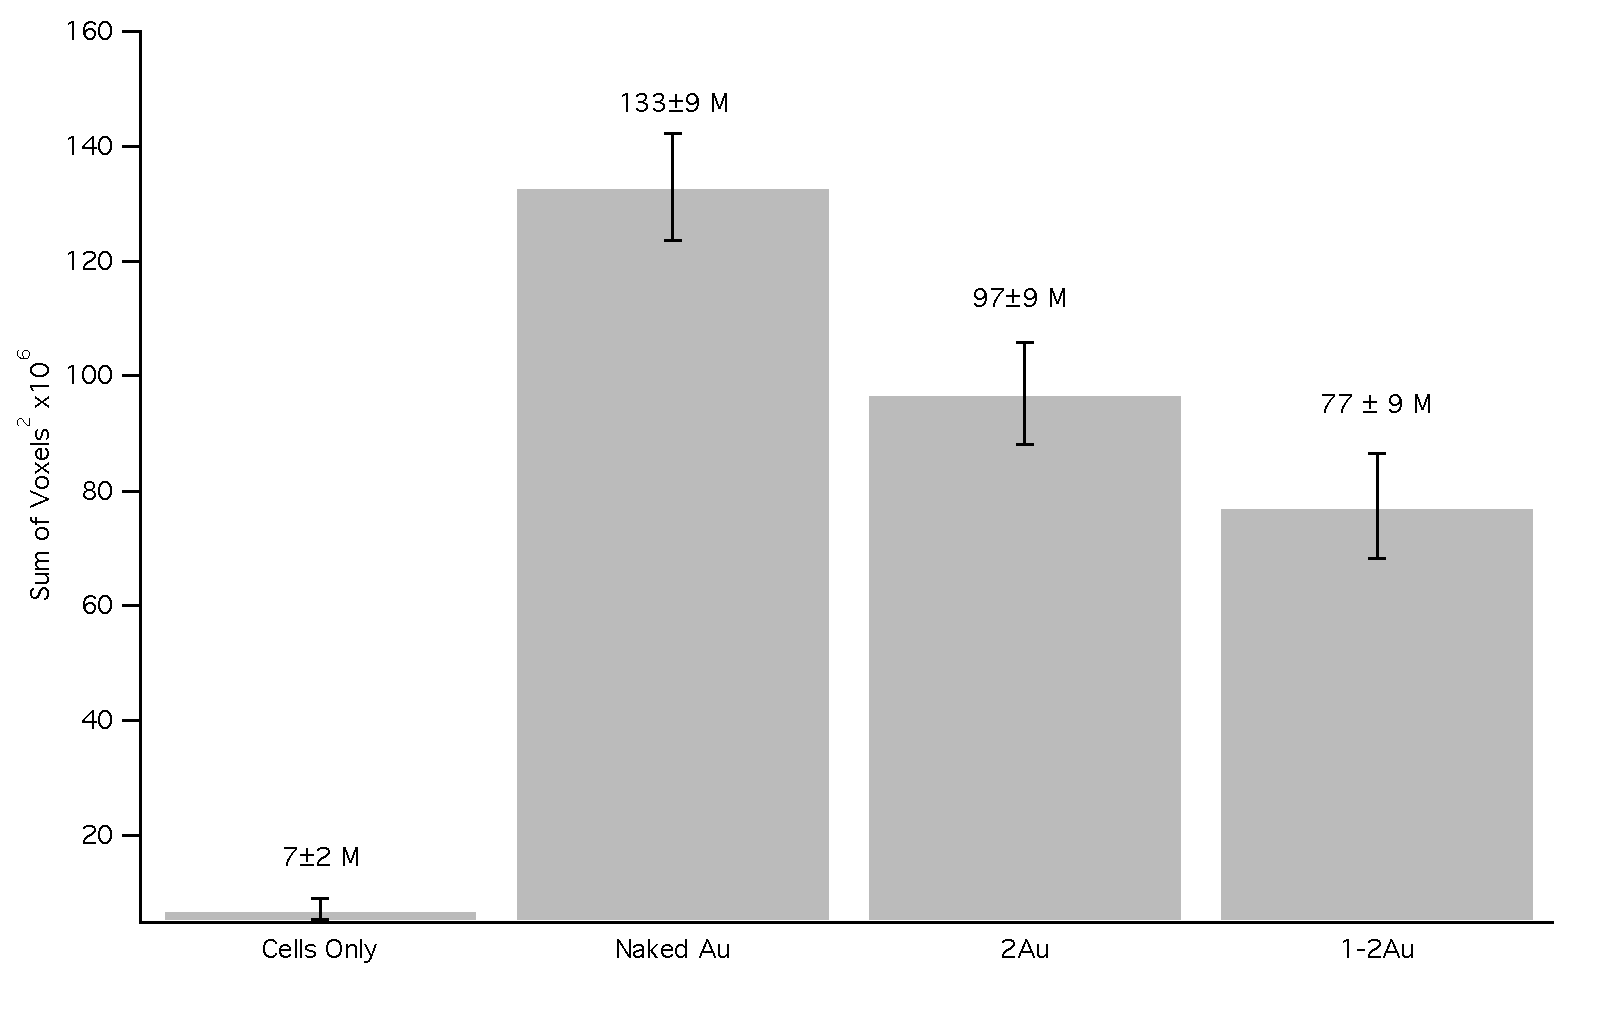
\includegraphics[keepaspectratio,width=\textwidth,height=0.75\textheight]{6marSOSgraph.pdf}
\caption{Sum of voxel values squared for gold-labeled preparations and unlabeled cells. Values are formed by taking the mean and standard error of sum of voxel values squared for each image corresponding to a given preparation.}
\label{marsosgraph}
\end{figure}



To quantify the amount of scattering increase, the sum of squares of the values of each voxel was tabulated for each OCM image. The mean and standard error of all the images from a given preparation were then calculated; those results are shown in \autoref{marsosgraph}. The increase in scattering in all three gold-labeled samples is shown quantitatively by comparing their sum of voxel values squared to that of the unlabeled cells. Among the gold-labeled samples themselves, the amount of scattering increase was the opposite of expected: the Au had the most scattering, then 2Au, then 1--2Au. However, the 2Au and 1--2Au samples are statistically indistinguishable.

The high amount of nonspecific binding was puzzling, and two hypotheses were put forth to explain the results of the labeling experiment. One possibility is that all of the spheres, especially the naked Au, bound to the cells via van der Waals forces. Because the naked Au has no dielectric separating it from whatever surface it comes in contact with, the strength of van der Waals forces will likely be much larger for the naked Au than for the 2Au. The second possibility concerns the use of Triton-X, a permeabilizing agent. Triton-X is used to permeabilize the cells so that the Sytox Green and phalloidin stains can diffuse inside the cell and stain the nucleus and actin cytoskeleton, respectively. Triton-X is a surfactant and permeablizes the cells by using surface tension to tear holes in the cell membrane. As a result, it was possible that the pores created by permeabilization of the cells allowed Au and 2Au to diffuse into the cell, but once in the cell, the gold nanospheres could not be removed by the washing process, leading to nonspecific contrast enhancement from nanoparticles inside the cell rather than on its surface. Furthermore, noting the strong background in some of the OCM images, there was some concern regarding the binding of the nanospheres to the coverslip surface itself. These concerns (van der Waals, permeabilization, and cover slip binding) led to a second round of immunolabeling experiments being performed on 3 April.

\begin{figure}[htbp]
\centering
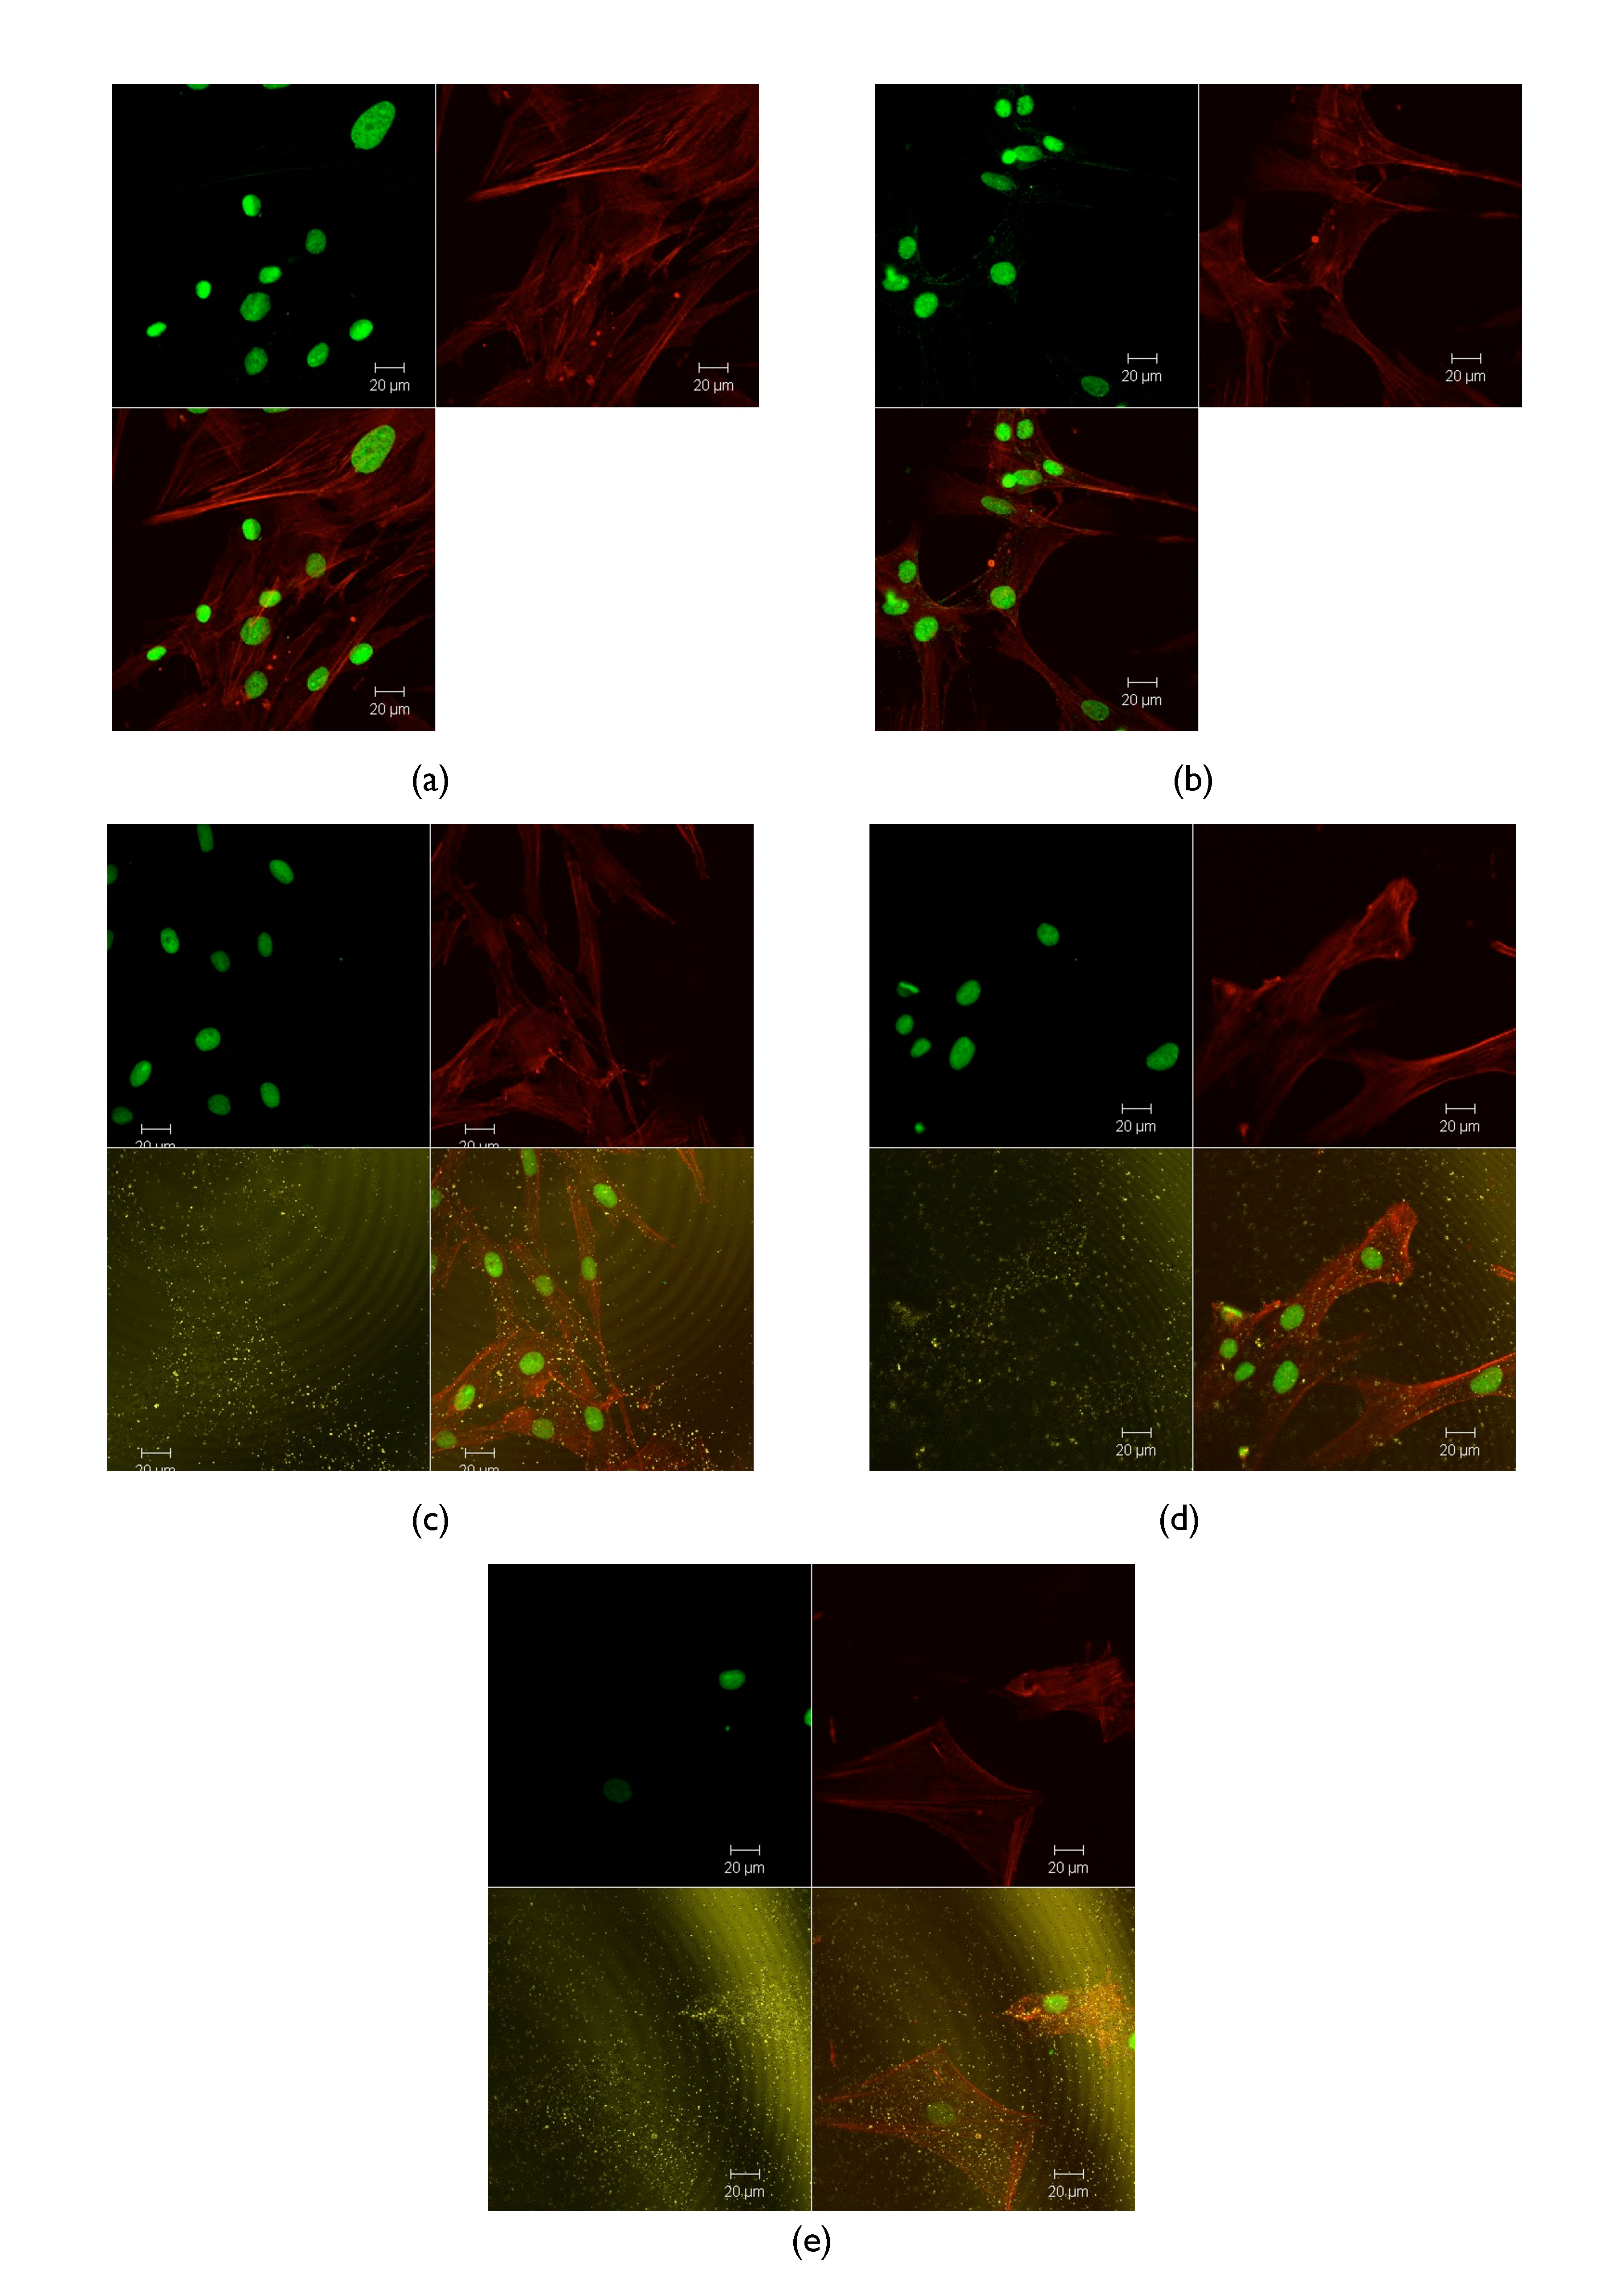
\includegraphics[keepaspectratio,width=\textwidth,height=9in]{ConfocalReps.pdf}
\caption{Confocal images of labeled preparations. Each image is a split view, showing Sytox and AP124F fluorescence (top left), phalloidin fluorescence (top right), backscattered light (c--e only; bottom left), and the composite view (bottom left, a and b; bottom right, c--e). Images correspond to preparations: (a) 2 only; (b) 1--2; (c) 1--2Au; (d) 2Au; (e) Au.}
\label{confocalcollage}
\end{figure}



\begin{figure}[htbp]
\centering
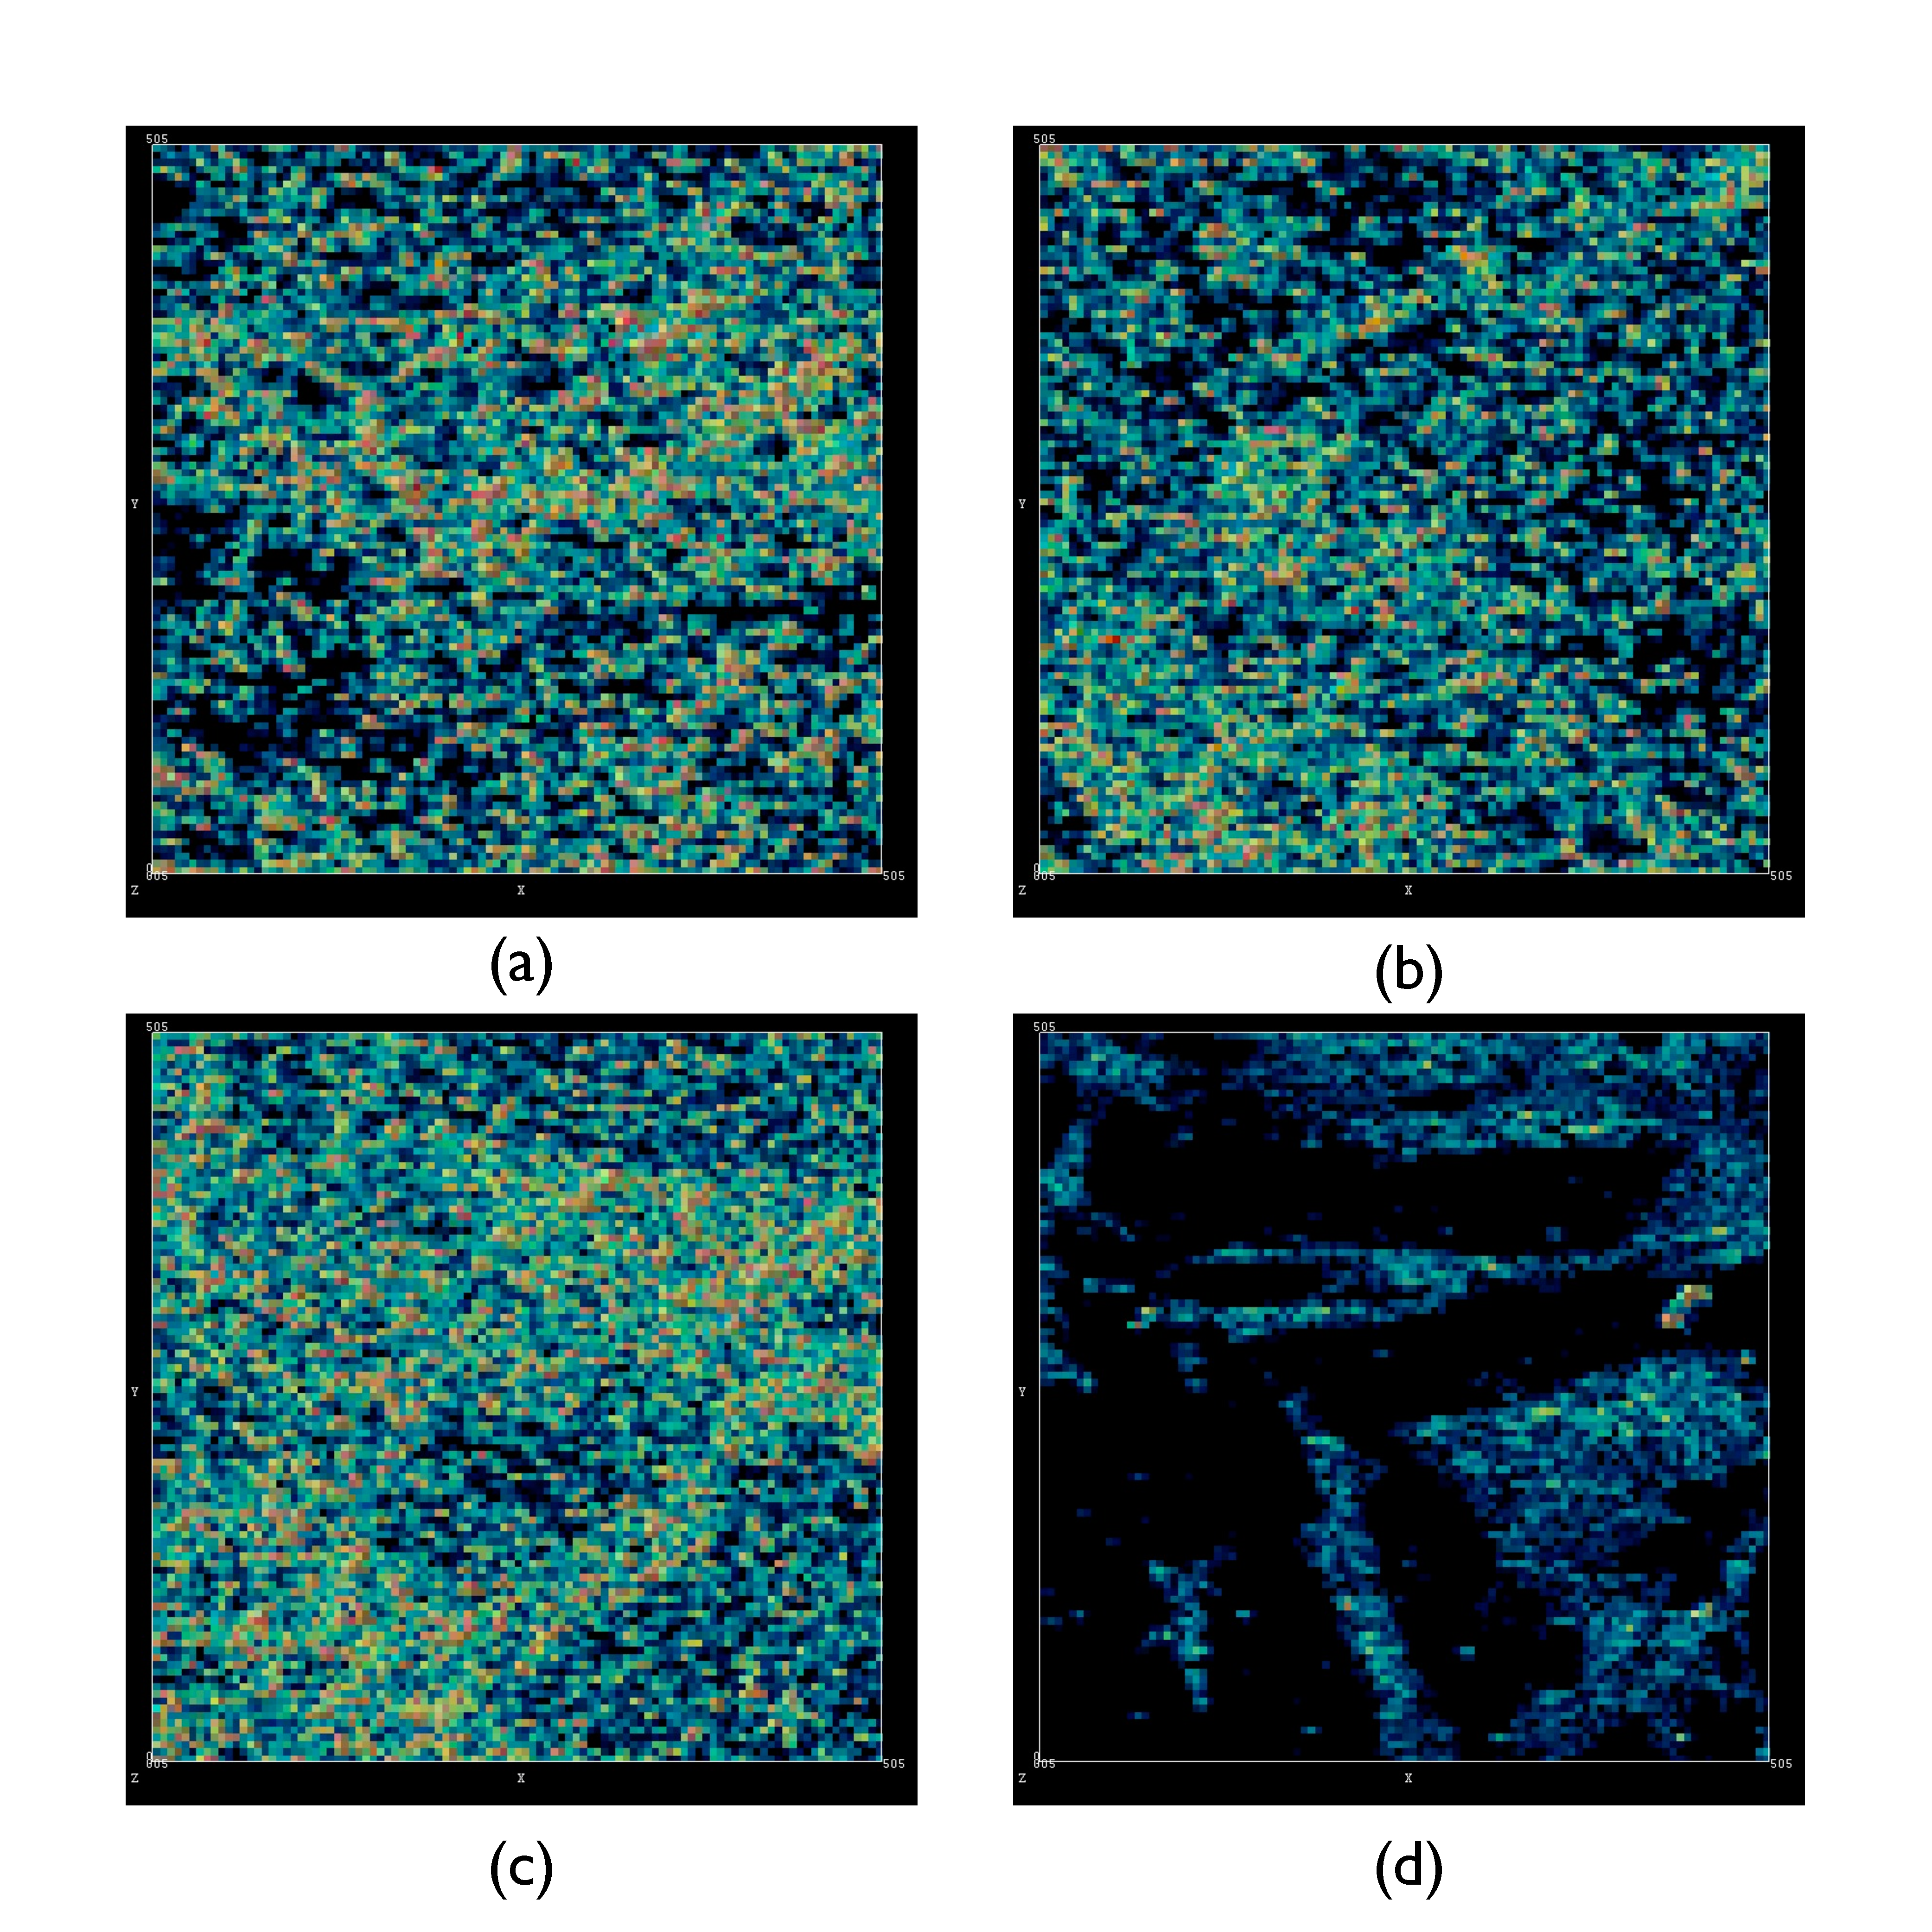
\includegraphics[keepaspectratio,width=\textwidth,height=0.75\textheight]{6marocmreprimages.pdf}
\caption{OCM images of labeled preparations. Images correspond to preparations: (a) 1--2Au; (b) 2Au; (c) Au; (d) Cells only.}
\label{marocmcollage}
\end{figure}

